%%
% Copyright (c) 2017 - 2024, Pascal Wagler;
% Copyright (c) 2014 - 2024, John MacFarlane
%
% All rights reserved.
%
% Redistribution and use in source and binary forms, with or without
% modification, are permitted provided that the following conditions
% are met:
%
% - Redistributions of source code must retain the above copyright
% notice, this list of conditions and the following disclaimer.
%
% - Redistributions in binary form must reproduce the above copyright
% notice, this list of conditions and the following disclaimer in the
% documentation and/or other materials provided with the distribution.
%
% - Neither the name of John MacFarlane nor the names of other
% contributors may be used to endorse or promote products derived
% from this software without specific prior written permission.
%
% THIS SOFTWARE IS PROVIDED BY THE COPYRIGHT HOLDERS AND CONTRIBUTORS
% "AS IS" AND ANY EXPRESS OR IMPLIED WARRANTIES, INCLUDING, BUT NOT
% LIMITED TO, THE IMPLIED WARRANTIES OF MERCHANTABILITY AND FITNESS
% FOR A PARTICULAR PURPOSE ARE DISCLAIMED. IN NO EVENT SHALL THE
% COPYRIGHT OWNER OR CONTRIBUTORS BE LIABLE FOR ANY DIRECT, INDIRECT,
% INCIDENTAL, SPECIAL, EXEMPLARY, OR CONSEQUENTIAL DAMAGES (INCLUDING,
% BUT NOT LIMITED TO, PROCUREMENT OF SUBSTITUTE GOODS OR SERVICES;
% LOSS OF USE, DATA, OR PROFITS; OR BUSINESS INTERRUPTION) HOWEVER
% CAUSED AND ON ANY THEORY OF LIABILITY, WHETHER IN CONTRACT, STRICT
% LIABILITY, OR TORT (INCLUDING NEGLIGENCE OR OTHERWISE) ARISING IN
% ANY WAY OUT OF THE USE OF THIS SOFTWARE, EVEN IF ADVISED OF THE
% POSSIBILITY OF SUCH DAMAGE.
%%

%%
% This is the Eisvogel pandoc LaTeX template.
%
% For usage information and examples visit the official GitHub page:
% https://github.com/Wandmalfarbe/pandoc-latex-template
%%

% Options for packages loaded elsewhere
\PassOptionsToPackage{unicode}{hyperref}
\PassOptionsToPackage{hyphens}{url}
\PassOptionsToPackage{dvipsnames,svgnames,x11names,table}{xcolor}
%
\documentclass[
  paper=a4,
  ,captions=tableheading
]{scrartcl}
\usepackage{amsmath,amssymb}
% Use setspace anyway because we change the default line spacing.
% The spacing is changed early to affect the titlepage and the TOC.
\usepackage{setspace}
\setstretch{1.2}
\usepackage{iftex}
\ifPDFTeX
  \usepackage[T1]{fontenc}
  \usepackage[utf8]{inputenc}
  \usepackage{textcomp} % provide euro and other symbols
\else % if luatex or xetex
  \usepackage{unicode-math} % this also loads fontspec
  \defaultfontfeatures{Scale=MatchLowercase}
  \defaultfontfeatures[\rmfamily]{Ligatures=TeX,Scale=1}
\fi
\usepackage{lmodern}
\ifPDFTeX\else
  % xetex/luatex font selection
\fi
% Use upquote if available, for straight quotes in verbatim environments
\IfFileExists{upquote.sty}{\usepackage{upquote}}{}
\IfFileExists{microtype.sty}{% use microtype if available
  \usepackage[]{microtype}
  \UseMicrotypeSet[protrusion]{basicmath} % disable protrusion for tt fonts
}{}
\makeatletter
\@ifundefined{KOMAClassName}{% if non-KOMA class
  \IfFileExists{parskip.sty}{%
    \usepackage{parskip}
  }{% else
    \setlength{\parindent}{0pt}
    \setlength{\parskip}{6pt plus 2pt minus 1pt}}
}{% if KOMA class
  \KOMAoptions{parskip=half}}
\makeatother
\usepackage{xcolor}
\definecolor{default-linkcolor}{HTML}{A50000}
\definecolor{default-filecolor}{HTML}{A50000}
\definecolor{default-citecolor}{HTML}{4077C0}
\definecolor{default-urlcolor}{HTML}{4077C0}
\usepackage[top=1.3in,bottom=1in]{geometry}
\usepackage{longtable,booktabs,array}
\usepackage{calc} % for calculating minipage widths
% Correct order of tables after \paragraph or \subparagraph
\usepackage{etoolbox}
\makeatletter
\patchcmd\longtable{\par}{\if@noskipsec\mbox{}\fi\par}{}{}
\makeatother
% Allow footnotes in longtable head/foot
\IfFileExists{footnotehyper.sty}{\usepackage{footnotehyper}}{\usepackage{footnote}}
\makesavenoteenv{longtable}
% add backlinks to footnote references, cf. https://tex.stackexchange.com/questions/302266/make-footnote-clickable-both-ways
\usepackage{footnotebackref}
\usepackage{graphicx}
\makeatletter
\newsavebox\pandoc@box
\newcommand*\pandocbounded[1]{% scales image to fit in text height/width
  \sbox\pandoc@box{#1}%
  \Gscale@div\@tempa{\textheight}{\dimexpr\ht\pandoc@box+\dp\pandoc@box\relax}%
  \Gscale@div\@tempb{\linewidth}{\wd\pandoc@box}%
  \ifdim\@tempb\p@<\@tempa\p@\let\@tempa\@tempb\fi% select the smaller of both
  \ifdim\@tempa\p@<\p@\scalebox{\@tempa}{\usebox\pandoc@box}%
  \else\usebox{\pandoc@box}%
  \fi%
}
% Set default figure placement to htbp
% Make use of float-package and set default placement for figures to H.
% The option H means 'PUT IT HERE' (as  opposed to the standard h option which means 'You may put it here if you like').
\usepackage{float}
\floatplacement{figure}{H}
\makeatother
\setlength{\emergencystretch}{3em} % prevent overfull lines
\providecommand{\tightlist}{%
  \setlength{\itemsep}{0pt}\setlength{\parskip}{0pt}}
\setcounter{secnumdepth}{-\maxdimen} % remove section numbering
\ifLuaTeX
\usepackage[bidi=basic]{babel}
\else
\usepackage[bidi=default]{babel}
\fi
\babelprovide[main,import]{english}
% get rid of language-specific shorthands (see #6817):
\let\LanguageShortHands\languageshorthands
\def\languageshorthands#1{}
\makeatletter
\@ifpackageloaded{subfig}{}{\usepackage{subfig}}
\@ifpackageloaded{caption}{}{\usepackage{caption}}
\captionsetup[subfloat]{margin=0.5em}
\AtBeginDocument{%
\renewcommand*\figurename{Figura}
\renewcommand*\tablename{Tabla}
}
\AtBeginDocument{%
\renewcommand*\listfigurename{Lista de Figuras}
\renewcommand*\listtablename{Lista de Tablas}
}
\newcounter{pandoccrossref@subfigures@footnote@counter}
\newenvironment{pandoccrossrefsubfigures}{%
\setcounter{pandoccrossref@subfigures@footnote@counter}{0}
\begin{figure}\centering%
\gdef\global@pandoccrossref@subfigures@footnotes{}%
\DeclareRobustCommand{\footnote}[1]{\footnotemark%
\stepcounter{pandoccrossref@subfigures@footnote@counter}%
\ifx\global@pandoccrossref@subfigures@footnotes\empty%
\gdef\global@pandoccrossref@subfigures@footnotes{{##1}}%
\else%
\g@addto@macro\global@pandoccrossref@subfigures@footnotes{, {##1}}%
\fi}}%
{\end{figure}%
\addtocounter{footnote}{-\value{pandoccrossref@subfigures@footnote@counter}}
\@for\f:=\global@pandoccrossref@subfigures@footnotes\do{\stepcounter{footnote}\footnotetext{\f}}%
\gdef\global@pandoccrossref@subfigures@footnotes{}}
\@ifpackageloaded{float}{}{\usepackage{float}}
\floatstyle{ruled}
\@ifundefined{c@chapter}{\newfloat{codelisting}{h}{lop}}{\newfloat{codelisting}{h}{lop}[chapter]}
\floatname{codelisting}{Listing}
\newcommand*\listoflistings{\listof{codelisting}{Listas del Documento}}
\makeatother
\usepackage{bookmark}
\IfFileExists{xurl.sty}{\usepackage{xurl}}{} % add URL line breaks if available
\urlstyle{same}
\hypersetup{
  pdfauthor={Versión actual: 1.aa3922c - Compilación para entrega - Mon, 9 Dec 2024 16:51:49 +0000},
  pdflang={en},
  pdfsubject={Implementación Proyecto JEP},
  pdfkeywords={Integración, Interoperabilidad, JEP, Softgic, Caso de
uso},
  hidelinks,
  breaklinks=true,
  pdfcreator={LaTeX via pandoc with the Eisvogel template}}
\usepackage{etoolbox}
\makeatletter
\providecommand{\subtitle}[1]{% add subtitle to \maketitle
  \apptocmd{\@title}{\par {\large #1 \par}}{}{}
}
\makeatother
\subtitle{Implementación Proyecto Evolución de Interoperabilidad JEP,
Softgic}
\author{Versión actual: 1.aa3922c - Compilación para entrega - Mon, 9
Dec 2024 16:51:49 +0000}
\date{2024-11-8}



%%
%% added
%%


%
% for the background color of the title page
%
\usepackage{pagecolor}
\usepackage{afterpage}

%
% break urls
%
\PassOptionsToPackage{hyphens}{url}

%
% When using babel or polyglossia with biblatex, loading csquotes is recommended
% to ensure that quoted texts are typeset according to the rules of your main language.
%
\usepackage{csquotes}

%
% captions
%
\definecolor{caption-color}{HTML}{777777}
\usepackage[font={stretch=1.2}, textfont={color=caption-color}, position=top, skip=4mm, labelfont=bf, singlelinecheck=false, justification=raggedright]{caption}
\setcapindent{0em}

%
% blockquote
%
\definecolor{blockquote-border}{RGB}{221,221,221}
\definecolor{blockquote-text}{RGB}{119,119,119}
\usepackage{mdframed}
\newmdenv[rightline=false,bottomline=false,topline=false,linewidth=3pt,linecolor=blockquote-border,skipabove=\parskip]{customblockquote}
\renewenvironment{quote}{\begin{customblockquote}\list{}{\rightmargin=0em\leftmargin=0em}%
\item\relax\color{blockquote-text}\ignorespaces}{\unskip\unskip\endlist\end{customblockquote}}

%
% Source Sans Pro as the default font family
% Source Code Pro for monospace text
%
% 'default' option sets the default
% font family to Source Sans Pro, not \sfdefault.
%
\ifnum 0\ifxetex 1\fi\ifluatex 1\fi=0 % if pdftex
    \usepackage[default]{sourcesanspro}
  \usepackage{sourcecodepro}
  \else % if not pdftex
    \usepackage[default]{sourcesanspro}
  \usepackage{sourcecodepro}

  % XeLaTeX specific adjustments for straight quotes: https://tex.stackexchange.com/a/354887
  % This issue is already fixed (see https://github.com/silkeh/latex-sourcecodepro/pull/5) but the
  % fix is still unreleased.
  % TODO: Remove this workaround when the new version of sourcecodepro is released on CTAN.
  \ifxetex
    \makeatletter
    \defaultfontfeatures[\ttfamily]
      { Numbers   = \sourcecodepro@figurestyle,
        Scale     = \SourceCodePro@scale,
        Extension = .otf }
    \setmonofont
      [ UprightFont    = *-\sourcecodepro@regstyle,
        ItalicFont     = *-\sourcecodepro@regstyle It,
        BoldFont       = *-\sourcecodepro@boldstyle,
        BoldItalicFont = *-\sourcecodepro@boldstyle It ]
      {SourceCodePro}
    \makeatother
  \fi
  \fi

%
% heading color
%
\definecolor{heading-color}{RGB}{40,40,40}
\addtokomafont{section}{\color{heading-color}}
% When using the classes report, scrreprt, book,
% scrbook or memoir, uncomment the following line.
%\addtokomafont{chapter}{\color{heading-color}}

%
% variables for title, author and date
%
\usepackage{titling}
\title{}
\author{Versión actual: 1.aa3922c - Compilación para entrega - Mon, 9
Dec 2024 16:51:49 +0000}
\date{2024-11-8}

%
% tables
%

\definecolor{table-row-color}{HTML}{F5F5F5}
\definecolor{table-rule-color}{HTML}{999999}

%\arrayrulecolor{black!40}
\arrayrulecolor{table-rule-color}     % color of \toprule, \midrule, \bottomrule
\setlength\heavyrulewidth{0.3ex}      % thickness of \toprule, \bottomrule
\renewcommand{\arraystretch}{1.3}     % spacing (padding)


%
% remove paragraph indentation
%
\setlength{\parindent}{0pt}
\setlength{\parskip}{6pt plus 2pt minus 1pt}
\setlength{\emergencystretch}{3em}  % prevent overfull lines

%
%
% Listings
%
%


%
% header and footer
%
\usepackage[headsepline,footsepline]{scrlayer-scrpage}

\newpairofpagestyles{eisvogel-header-footer}{
  \clearpairofpagestyles
  \ihead*{2024-11-8}
  \chead*{}
  \ohead*{
\includegraphics{include/jeplogo.jpg}}
  \ifoot*{Versión actual: 1.aa3922c - Compilación para entrega - Mon, 9
Dec 2024 16:51:49 +0000}
  \cfoot*{}
  \ofoot*{\thepage}
  \addtokomafont{pageheadfoot}{\upshape}
}
\pagestyle{eisvogel-header-footer}



%%
%% end added
%%

\begin{document}

%%
%% begin titlepage
%%
\begin{titlepage}
\newgeometry{left=6cm}
\newcommand{\colorRule}[3][black]{\textcolor[HTML]{#1}{\rule{#2}{#3}}}
\begin{flushleft}
\noindent
\\[-1em]
\color[HTML]{5F5F5F}
\makebox[0pt][l]{\colorRule[360049]{1.3\textwidth}{4pt}}
\par
\noindent

{
  \setstretch{1.4}
  \vfill
  \noindent {\huge \textbf{\textsf{}}}
    \vskip 1em
  {\Large \textsf{Implementación Proyecto Evolución de Interoperabilidad
JEP, Softgic}}
    \vskip 2em
  \noindent {\Large \textsf{Versión actual: 1.aa3922c - Compilación para
entrega - Mon, 9 Dec 2024 16:51:49 +0000}}
  \vfill
}


\textsf{2024-11-8}
\end{flushleft}
\end{titlepage}
\restoregeometry
\pagenumbering{arabic}

%%
%% end titlepage
%%



\section{Especificación CU Requerimiento
REQR17}\label{sec:especificaciuxf3n-cu-requerimiento-reqr17}

\begin{itemize}
\tightlist
\item
  \hyperref[Introducciuxf3n]{Introducción}
\item
  \hyperref[reqr17.-integraciuxf3n-conti---comparecientes-requirement]{REQR17.
  Integración Conti - Comparecientes (Requirement)}

  \begin{itemize}
  \tightlist
  \item
    \hyperref[hu.sint80.-integraciuxf3n-gettoken-deliverable]{HU.SINT80.
    Integración getToken (Deliverable)}

    \begin{itemize}
    \tightlist
    \item
      \hyperref[especificaciuxf3n-de-integraciuxf3n-deliverable]{Especificación
      de integración (Deliverable)}
    \end{itemize}
  \item
    \hyperref[hu.sint81.-integraciuxf3n-consulta-radicado-deliverable]{HU.SINT81.
    Integración Consulta radicado (Deliverable)}

    \begin{itemize}
    \tightlist
    \item
      \hyperref[especificaciuxf3n-de-integraciuxf3n-deliverable-2]{Especificación
      de integración (Deliverable) 2}
    \end{itemize}
  \item
    \hyperref[hu.sint82.-integraciuxf3n-consulta-acta-deliverable]{HU.SINT82.
    Integración Consulta acta (Deliverable)}

    \begin{itemize}
    \tightlist
    \item
      \hyperref[especificaciuxf3n-de-integraciuxf3n-deliverable-3]{Especificación
      de integración (Deliverable) 3}
    \end{itemize}
  \end{itemize}
\end{itemize}

\subsection{Introducción}\label{sec:introducciuxf3n}

\begin{figure}
\centering
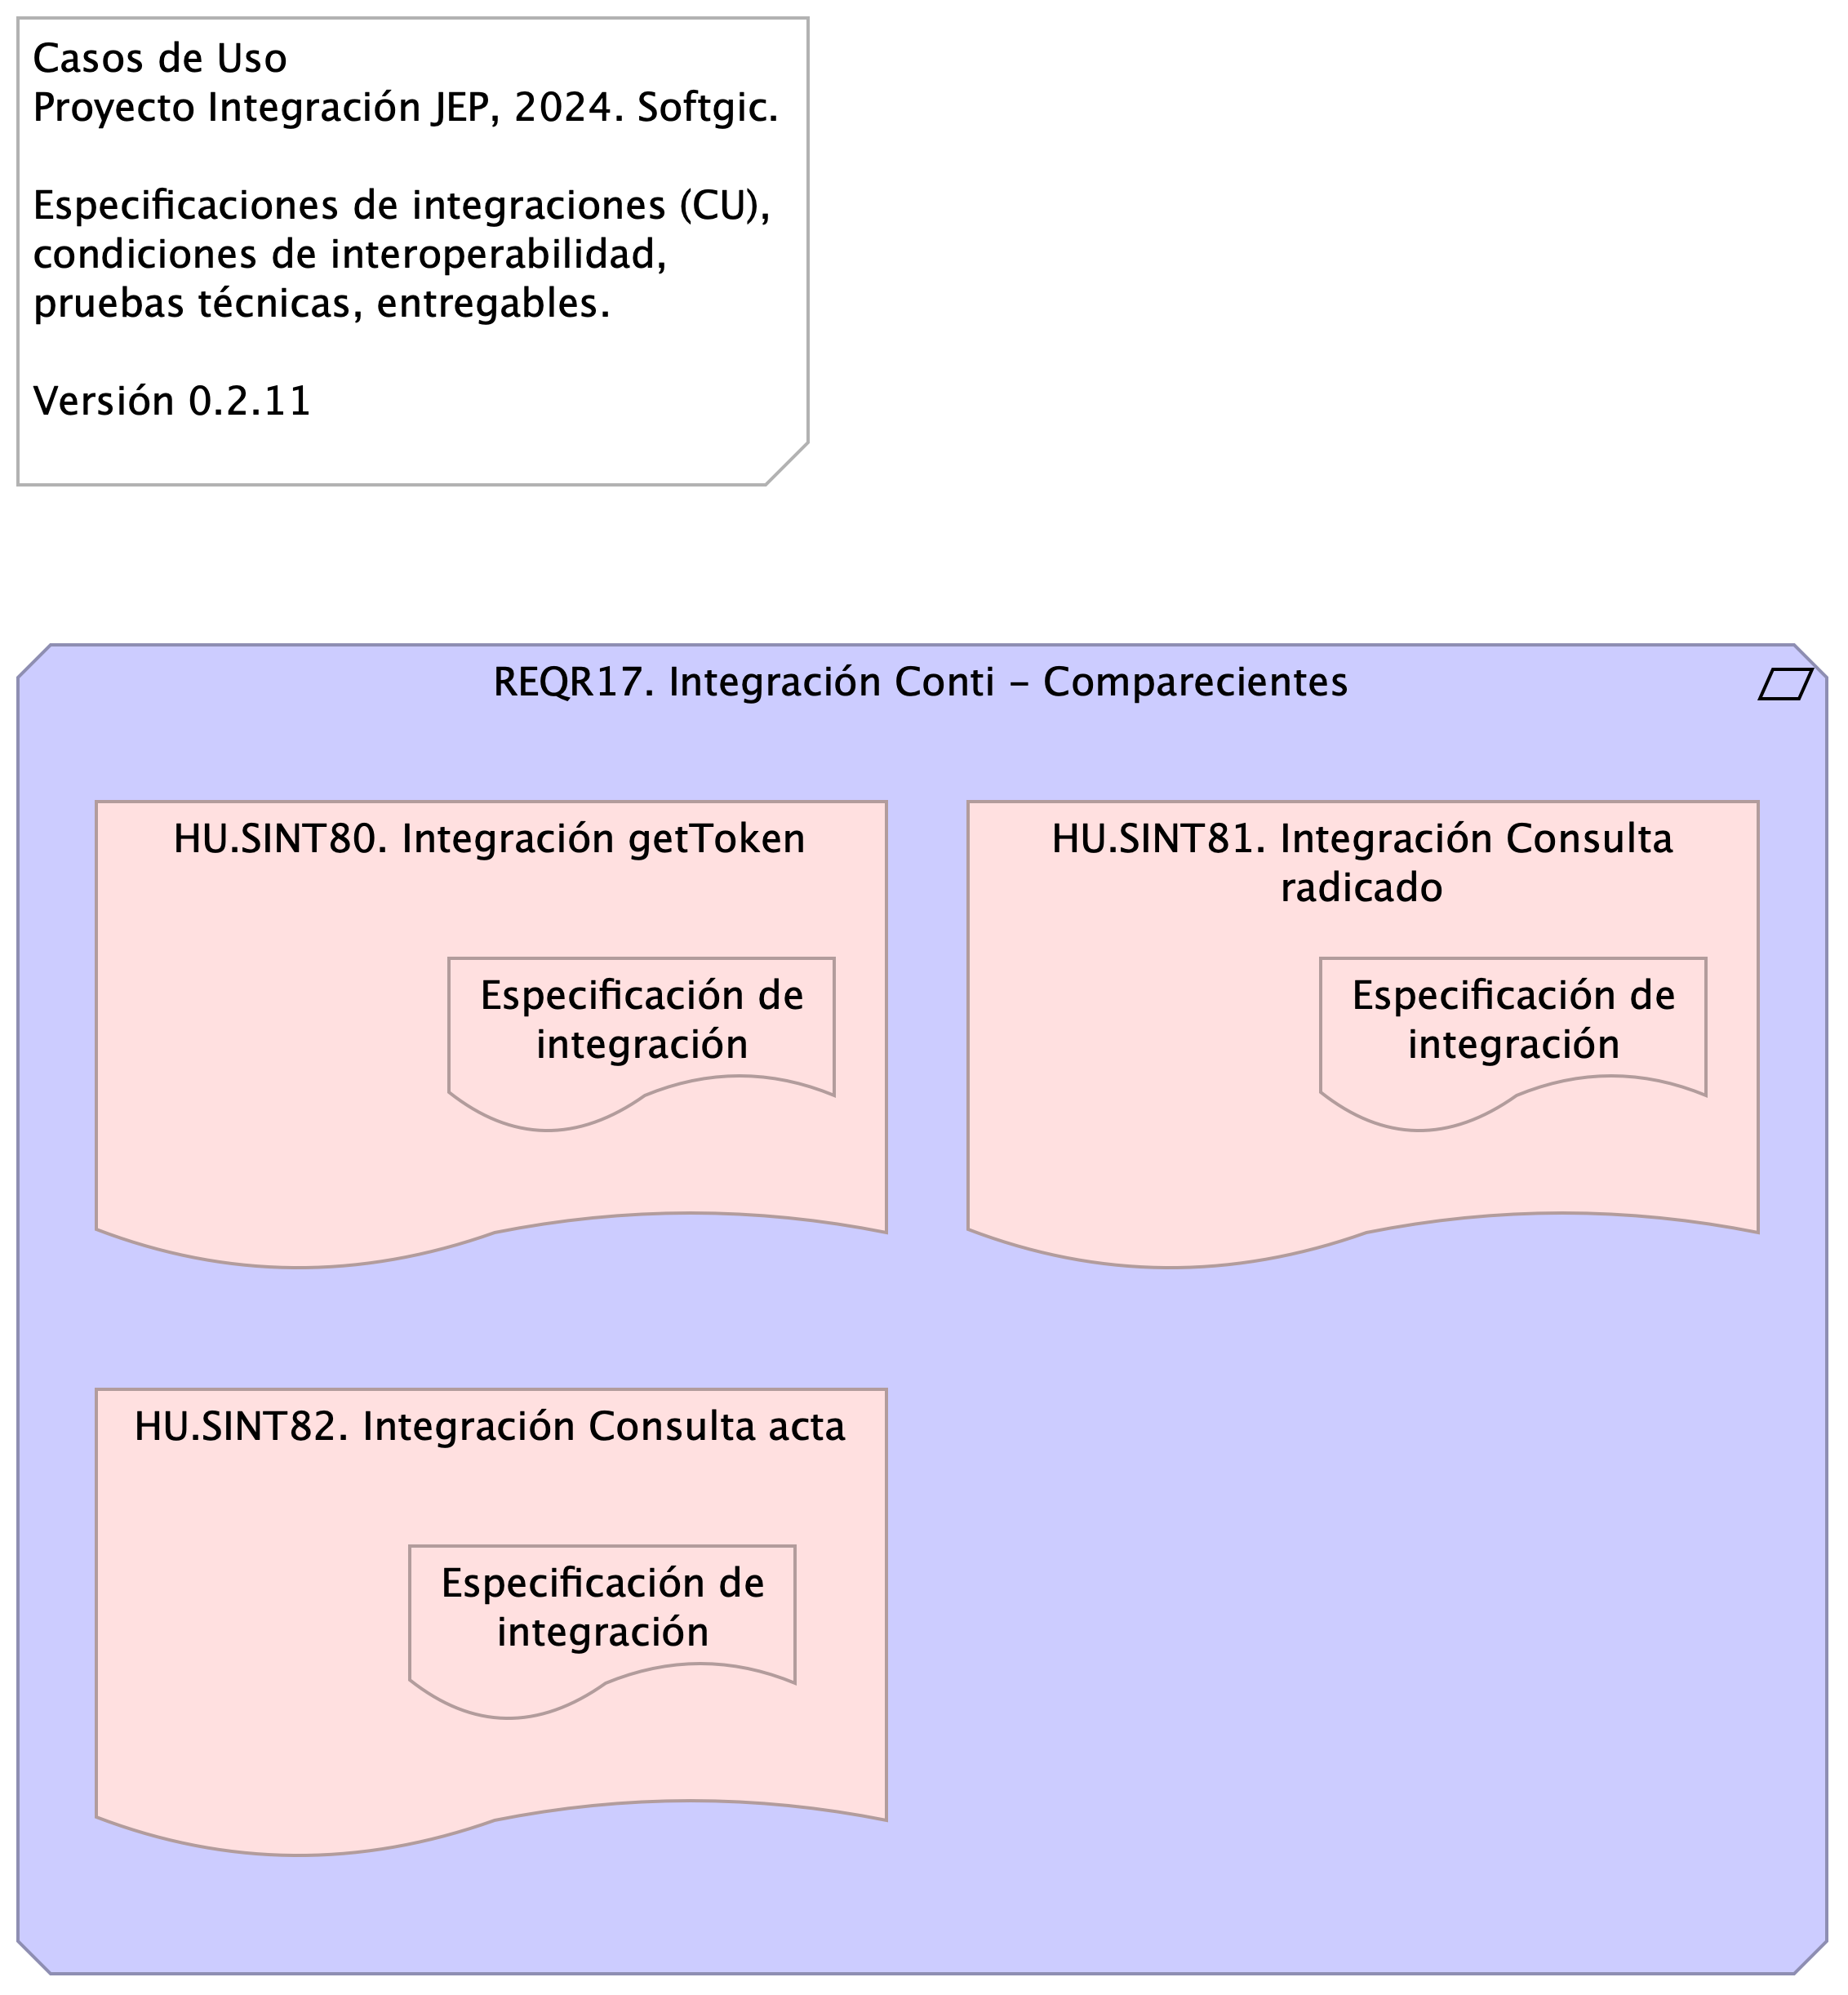
\includegraphics[width=\textwidth,height=5.20833in]{03.cu.reqr17.png}
\caption{05.REQR.2n.6n. Casos de Uso REQR17}
\end{figure}

Documentación de los casos de uso de integración del proyecto JEP
relacionados con los requerimientos. COndiciones de interoperabilidad,
pruebas técnicas y entregables.

Fuente: Acta de requerimientos Integración Plani - Proceso
Precontractual\_V4.pdf

\subsection{REQR17. Integración Conti -
Comparecientes}\label{sec:reqr17.-integraciuxf3n-conti---comparecientes}

Atendiendo la necesidad de Justicia Digital, se requiere implementar la
integración con el módjlos de comparecientes de Conti, como la
exposición de las capacidades de Conti.

Fuente: serviciosOami (pdf).

\subsubsection{Índice de la documentación (casos de
uso)}\label{sec:uxedndice-de-la-documentaciuxf3n-casos-de-uso}

\begin{enumerate}
\def\labelenumi{\arabic{enumi}.}
\tightlist
\item
  SINT80. Integrar getToken
\item
  SINT81. Integrar Consulta radicado
\item
  SINT82. Integrar Consulta acta
\end{enumerate}

Los casos de uso se detallan en anexo más adelante.

\subsubsection{HU.SINT80. Integración
getToken}\label{sec:hu.sint80.-integraciuxf3n-gettoken}

\paragraph{Especificación de
integración}\label{sec:especificaciuxf3n-de-integraciuxf3n}

Integrar el servicio que retorna token de autenticación para los demás
servicios, getToken de Conti y devolver resultado al módulo de
comparecientes.

\paragraph{Elementos}\label{sec:elementos}

Elegir y describir los elementos de la actual integración.

\begin{itemize}
\tightlist
\item[$\boxtimes$]
  App consumidora (A)
\item[$\boxtimes$]
  Mensaje
\item[$\square$]
  Canal
\item[$\square$]
  Ruteo
\item[$\square$]
  Traducción
\item[$\boxtimes$]
  App proveedora (B)
\item[$\square$]
  Monitoreo
\end{itemize}

Aplicación consumidora A: Comparecientes. Aplicación proveedora B: Conti

Mensaje solicitud: (ver estándar de nombramiento) Ingreso a Conti

\begin{itemize}
\tightlist
\item
  Tipo: TXT \textbar{} SOAP \textbar{} XML \textbar{} JSN \textbar{} YML
  \textbar{} BASE64
\item
  Contenido: Token de seguridad para la autorización de la operación en
  el módulo de comparecientes.
\end{itemize}

Mensaje respuesta: Rpta. Token de autorización

\begin{itemize}
\tightlist
\item
  Tipo: TXT \textbar{} SOAP \textbar{} XML \textbar{} JSN \textbar{} YML
  \textbar{} BASE64
\item
  Contenido: Estado de solicitud de ingreso a Conti
\end{itemize}

Mensaje excepción: Rpta. Token no válido

\begin{itemize}
\tightlist
\item
  Tipo: TXT \textbar{} SOAP \textbar{} XML \textbar{} JSN \textbar{} YML
  \textbar{} BASE64
\item
  Contenido: Código de respuesta: HTTP 500 \textbar{} TXT \textbar{}
  Numeración (entero)
\end{itemize}

\paragraph{Diseño}\label{sec:diseuxf1o}

Message Construct \textbar{} Message Routing \textbar{} Message
Transformation \textbar{} Messaging Endpoints \textbar{} Messaging
Channels \textbar{} \ldots{}

La aplicación consumidora y proveedora compartirán capacidades mediante
un mensaje de autorización (Message Construct).

\paragraph{Puntos de Entrada (endpoints) Aplicación
Proveedora}\label{sec:puntos-de-entrada-endpoints-aplicaciuxf3n-proveedora}

\begin{itemize}
\tightlist
\item
  Url: dominio/mercurio/apiRest/consulta/getToken
\item
  Method: POST
\item
  Content-Type: application/json
\end{itemize}

\paragraph{Matriz de
interoperabilidad}\label{sec:matriz-de-interoperabilidad}

Detalle del intercambio entre sistemas de información o aplicaciones.

App Plani requiere compartir Información {[}I{]}, Funcionalidad {[}F{]},
Seguridad o Servicios {[}S{]} con la App Plani.

\begin{longtable}[]{@{}lllll@{}}
\caption{Matriz de interoperabilidad del CU getToken}\tabularnewline
\toprule\noalign{}
& Conti & Comparecientes & Legali & Otros \\
\midrule\noalign{}
\endfirsthead
\toprule\noalign{}
& Conti & Comparecientes & Legali & Otros \\
\midrule\noalign{}
\endhead
\bottomrule\noalign{}
\endlastfoot
Conti (A) & X & Seguridad & & \\
Comparecientes (B) & & X & & \\
Legali & & & X & \\
Otros Sistemas & & & & X \\
\end{longtable}

\paragraph{Pruebas Realizables}\label{sec:pruebas-realizables}

Por cada caso de prueba de integración describir el resultado del
intercambio entre sistemas de información o aplicaciones según la Matriz
de interoperabilidad.

\begin{itemize}
\tightlist
\item
  PRUB1. Token: la aplicación consumidora solicita un token de
  autorización.
\item
  PRUB2. Falla Token: la aplicación proveedora Conti no provee el token
  de autorización.
\end{itemize}

\paragraph{Anexo Técnico}\label{sec:anexo-tuxe9cnico}

Manual de especificación de los servicios web. ServiciosOami.pdf

\subsubsection{HU.SINT81. Integración Consulta
radicado}\label{sec:hu.sint81.-integraciuxf3n-consulta-radicado}

\paragraph{Especificación de
integración}\label{sec:especificaciuxf3n-de-integraciuxf3n-1}

Integrar el servicio REST que retorna información asociada a los
radicados que almacena Conti, consulta\_radicado de Conti y devolver
resultado al módulo de comparecientes.

El servicio

\paragraph{Elementos}\label{sec:elementos-1}

Elegir y describir los elementos de la actual integración.

\begin{itemize}
\tightlist
\item[$\boxtimes$]
  App consumidora (A)
\item[$\boxtimes$]
  Mensaje
\item[$\square$]
  Canal
\item[$\square$]
  Ruteo
\item[$\square$]
  Traducción
\item[$\boxtimes$]
  App proveedora (B)
\item[$\square$]
  Monitoreo
\end{itemize}

Aplicación consumidora A: Comparecientes. Aplicación proveedora B: Conti

Mensaje solicitud: (ver estándar de nombramiento) Ingreso a Conti

\begin{itemize}
\tightlist
\item
  Tipo: TXT \textbar{} SOAP \textbar{} XML \textbar{} JSN \textbar{} YML
  \textbar{} BASE64
\item
  Contenido: Token de seguridad para la autorización de la operación en
  el módulo de comparecientes.
\end{itemize}

Mensaje respuesta: Rpta. Token de autorización

\begin{itemize}
\tightlist
\item
  Tipo: TXT \textbar{} SOAP \textbar{} XML \textbar{} JSN \textbar{} YML
  \textbar{} BASE64
\item
  Contenido: Estado de solicitud de ingreso a Conti
\end{itemize}

Mensaje excepción: Rpta. Token no válido

\begin{itemize}
\tightlist
\item
  Tipo: TXT \textbar{} SOAP \textbar{} XML \textbar{} JSN \textbar{} YML
  \textbar{} BASE64
\item
  Contenido: Código de respuesta: HTTP 500 \textbar{} TXT \textbar{}
  Numeración (entero)
\end{itemize}

\paragraph{Diseño}\label{sec:diseuxf1o-1}

Message Construct \textbar{} Message Routing \textbar{} Message
Transformation \textbar{} Messaging Endpoints \textbar{} Messaging
Channels \textbar{} \ldots{}

La aplicación consumidora y proveedora compartirán capacidades mediante
un mensaje de autorización (Message Construct).

\paragraph{Puntos de Entrada (endpoints) Aplicación
Proveedora}\label{sec:puntos-de-entrada-endpoints-aplicaciuxf3n-proveedora-1}

\begin{itemize}
\tightlist
\item
  Url: dominio/mercurio/apiRest/consulta/contenidoradicado
\item
  Method: POST
\item
  Content-Type: application/json
\item
  Authorization: Bearer Token
\end{itemize}

\paragraph{Matriz de
interoperabilidad}\label{sec:matriz-de-interoperabilidad-1}

Detalle del intercambio entre sistemas de información o aplicaciones.

App Plani requiere compartir Información {[}I{]}, Funcionalidad {[}F{]},
Seguridad o Servicios {[}S{]} con la App Plani.

\begin{longtable}[]{@{}lllll@{}}
\caption{Matriz de interoperabilidad del CU getToken}\tabularnewline
\toprule\noalign{}
& Conti & Comparecientes & Legali & Otros \\
\midrule\noalign{}
\endfirsthead
\toprule\noalign{}
& Conti & Comparecientes & Legali & Otros \\
\midrule\noalign{}
\endhead
\bottomrule\noalign{}
\endlastfoot
Conti (A) & X & Seguridad & & \\
Comparecientes (B) & & X & & \\
Legali & & & X & \\
Otros Sistemas & & & & X \\
\end{longtable}

\paragraph{Pruebas Realizables}\label{sec:pruebas-realizables-1}

Por cada caso de prueba de integración describir el resultado del
intercambio entre sistemas de información o aplicaciones según la Matriz
de interoperabilidad.

\begin{itemize}
\tightlist
\item
  PRUB1. Token: la aplicación consumidora solicita un token de
  autorización.
\item
  PRUB2. Falla Token: la aplicación proveedora Conti no provee el token
  de autorización.
\end{itemize}

\paragraph{Anexo Técnico}\label{sec:anexo-tuxe9cnico-1}

Manual de especificación de los servicios web. ServiciosOami.pdf

\subsubsection{HU.SINT82. Integración Consulta
acta}\label{sec:hu.sint82.-integraciuxf3n-consulta-acta}

\paragraph{Especificación de
integración}\label{sec:especificaciuxf3n-de-integraciuxf3n-2}

Integrar el servicio que retorna información asociada a las actas que
almacena Conti, consulta Acta de Conti y devolver resultado al módulo de
comparecientes.

El servicio

\paragraph{Elementos}\label{sec:elementos-2}

Elegir y describir los elementos de la actual integración.

\begin{itemize}
\tightlist
\item[$\boxtimes$]
  App consumidora (A)
\item[$\boxtimes$]
  Mensaje
\item[$\square$]
  Canal
\item[$\square$]
  Ruteo
\item[$\square$]
  Traducción
\item[$\boxtimes$]
  App proveedora (B)
\item[$\square$]
  Monitoreo
\end{itemize}

Aplicación consumidora A: Comparecientes. Aplicación proveedora B: Conti

Mensaje solicitud: (ver estándar de nombramiento) Ingreso a Conti

\begin{itemize}
\tightlist
\item
  Tipo: TXT \textbar{} SOAP \textbar{} XML \textbar{} JSN \textbar{} YML
  \textbar{} BASE64
\item
  Contenido: Token de seguridad para la autorización de la operación en
  el módulo de comparecientes.
\end{itemize}

Mensaje respuesta: Rpta. Token de autorización

\begin{itemize}
\tightlist
\item
  Tipo: TXT \textbar{} SOAP \textbar{} XML \textbar{} JSN \textbar{} YML
  \textbar{} BASE64
\item
  Contenido: Estado de solicitud de ingreso a Conti
\end{itemize}

Mensaje excepción: Rpta. Token no válido

\begin{itemize}
\tightlist
\item
  Tipo: TXT \textbar{} SOAP \textbar{} XML \textbar{} JSN \textbar{} YML
  \textbar{} BASE64
\item
  Contenido: Código de respuesta: HTTP 500 \textbar{} TXT \textbar{}
  Numeración (entero)
\end{itemize}

\paragraph{Diseño}\label{sec:diseuxf1o-2}

Message Construct \textbar{} Message Routing \textbar{} Message
Transformation \textbar{} Messaging Endpoints \textbar{} Messaging
Channels \textbar{} \ldots{}

La aplicación consumidora y proveedora compartirán capacidades mediante
un mensaje de autorización (Message Construct).

\paragraph{Puntos de Entrada (endpoints) de Aplicación
Proveedora}\label{sec:puntos-de-entrada-endpoints-de-aplicaciuxf3n-proveedora}

\begin{itemize}
\tightlist
\item
  Url: dominio/mercurio/apiRest/consulta/acta
\item
  Method: POST
\item
  Content-Type: application/json
\item
  Authorization: Bearer Token
\end{itemize}

\paragraph{Matriz de
interoperabilidad}\label{sec:matriz-de-interoperabilidad-2}

Detalle del intercambio entre sistemas de información o aplicaciones.

App Plani requiere compartir Información {[}I{]}, Funcionalidad {[}F{]},
Seguridad o Servicios {[}S{]} con la App Plani.

\begin{longtable}[]{@{}lllll@{}}
\caption{Matriz de interoperabilidad del CU getToken}\tabularnewline
\toprule\noalign{}
& Conti & Comparecientes & Legali & Otros \\
\midrule\noalign{}
\endfirsthead
\toprule\noalign{}
& Conti & Comparecientes & Legali & Otros \\
\midrule\noalign{}
\endhead
\bottomrule\noalign{}
\endlastfoot
Conti (A) & X & Seguridad & & \\
Comparecientes (B) & & X & & \\
Legali & & & X & \\
Otros Sistemas & & & & X \\
\end{longtable}

\paragraph{Pruebas Realizables}\label{sec:pruebas-realizables-2}

Por cada caso de prueba de integración describir el resultado del
intercambio entre sistemas de información o aplicaciones según la Matriz
de interoperabilidad.

\begin{itemize}
\tightlist
\item
  PRUB1. Consulta acta: la aplicación consumidora solicita y recibe el
  acta solicitada.
\item
  PRUB2. Acta no existe: la aplicación proveedora Conti no provee el
  acta solicitada.
\end{itemize}

\paragraph{Anexo Técnico}\label{sec:anexo-tuxe9cnico-2}

Manual de especificación de los servicios web. ServiciosOami.pdf

\end{document}
